\documentclass[12pt]{report}
\usepackage[utf8]{inputenc}
\usepackage{cite}
\usepackage[hidelinks]{hyperref}
\usepackage{graphicx}
\usepackage{amsfonts}
\usepackage{mathtools}
\usepackage{caption}
\usepackage{fancyhdr}

\pagestyle{fancy}
\fancyhf{}
\rhead{5-stage Pipelined Processor Design Report}
\lhead{\thesection}
\rfoot{\thepage}

\DeclarePairedDelimiter\ceil{\lceil}{\rceil}
\DeclarePairedDelimiter\floor{\lfloor}{\rfloor}

\title{\textbf{5-stage Pipelined Processor Design Report}\\Team \#4}
\author{
  Mohamed Shawky\\
  \small\texttt{SEC:2, BN:16}
  \and
  Remonda Talaat\\
  \small\texttt{SEC:1, BN:20}
  \and
  Evram Youssef\\
  \small\texttt{SEC:1, BN:9}
  \and
  Mahmoud Adas\\
  \small\texttt{SEC:2, BN:21}
}
\date{\today}

\begin{document}

\thispagestyle{empty}

\maketitle
\tableofcontents
\listoffigures
\listoftables
\clearpage

\pagenumbering{arabic}

\part{Introduction}

\part{Overall System}

\section{Overall Design Schema}
\begin{center}
    \begin{figure}[hp]
        \centering
        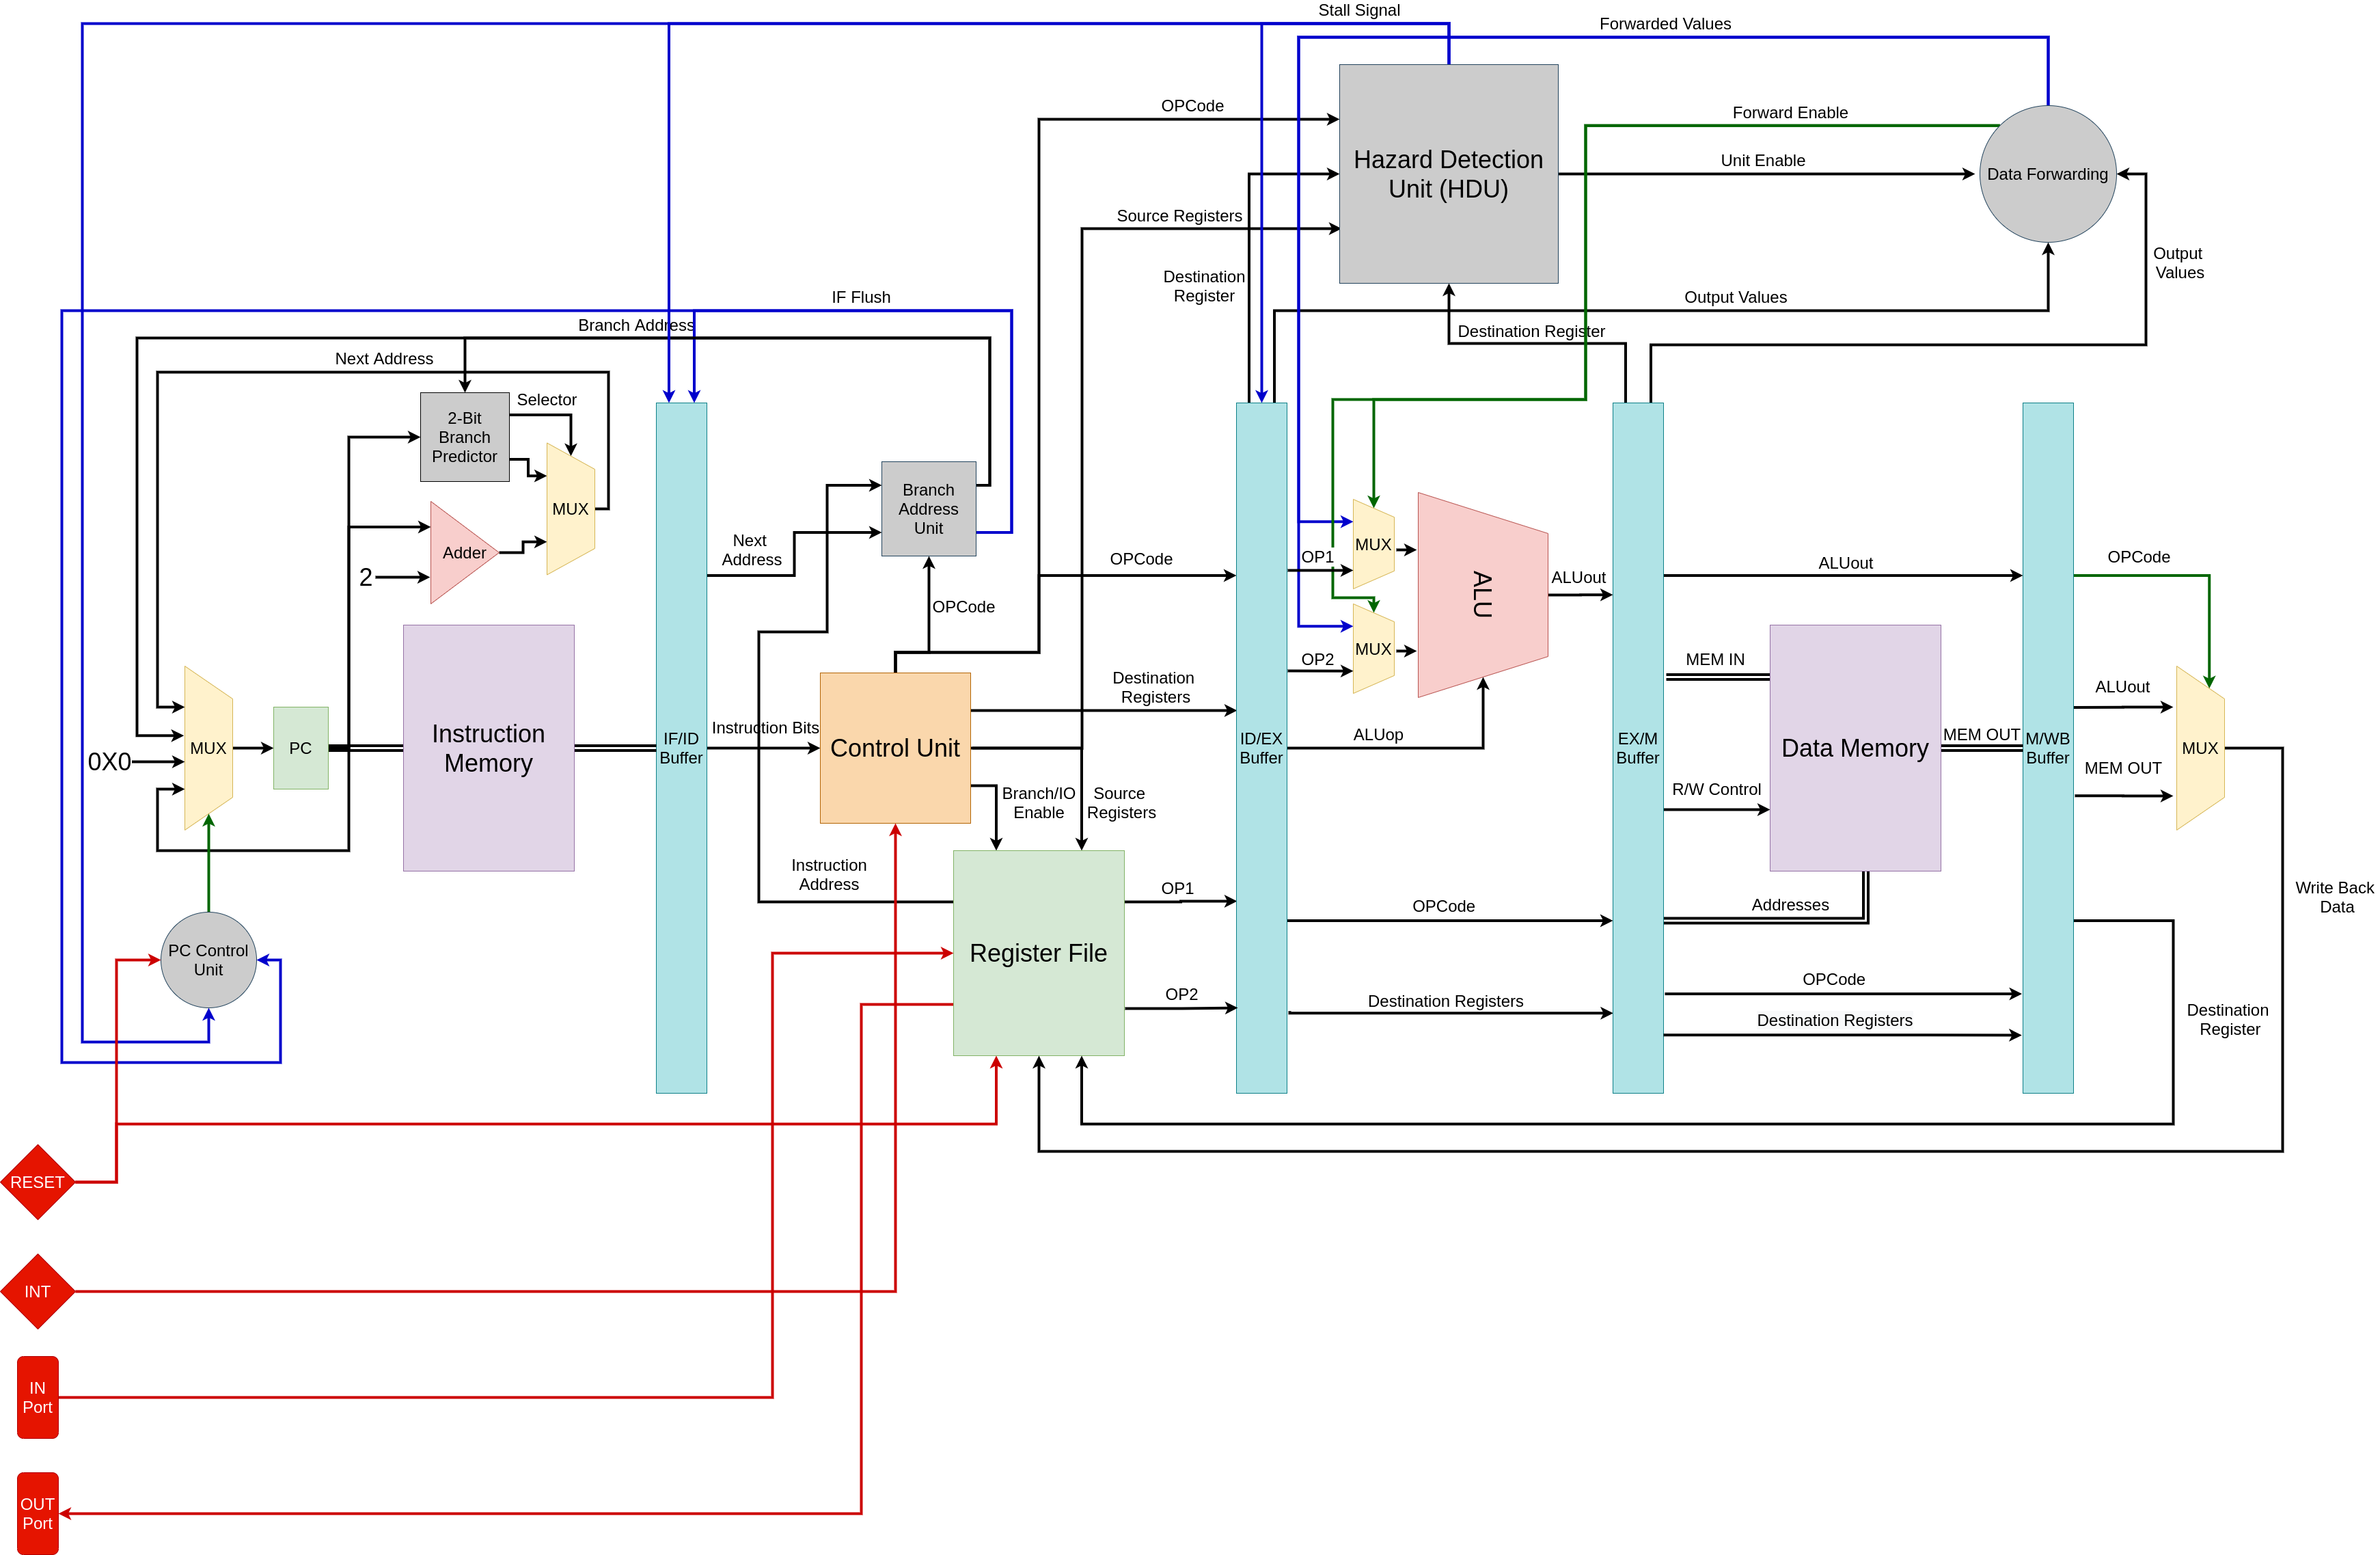
\includegraphics[width=\textwidth]{overall_system}
        \caption{Overall System Design}
        \label{fig:overall}
    \end{figure}
\end{center}

\section{Hazards Detection}

\subsection{Structural Hazards}
No detection required.

\subsection{Data Hazards}
Refer the \emph{HDU} in \ref{fig:overall}

\subsection{Control Hazards}
\begin{itemize}
    \item At Fetch stage, always check the branch predictor and calculate the next address accordingly.
    \item At Decode stage, check whether the OPCode is of a branch operation. If so, pass the address to the program counter and compare the correct address with the address of the counter to decide whether to flush the Fetch stage or not. 
\end{itemize}

\section{Hazards Handling}

\subsection{Structural Hazards}
2 memory units, one for instructions and one for data. Both have the same specs \emph{(mentioned below)}. \\
Also, to handle register file structural hazard, the write back will be in the first half of the clock cycle and the decode will be in the second half.

\subsection{Data Hazards}

\subsubsection{Stall}
Occurs only at Decode stage, due to load use case.
\begin{itemize}
    \item Fetch same instruction (don't increment the program counter).
    \item Latch IF/ID buffer with the same values.
    \item Freeze Decode stage.
    \item Clear ID/EX buffer.
\end{itemize}

\subsubsection{Data Forwarding}
\begin{itemize}
    \item EX/MEM buffer $->$ Execute / Decode.
    \item ID/EX buffer $->$ Decode.
\end{itemize}

\subsection{Control Hazards}

\subsubsection{Flush}
Occurs only at Fetch Stage, due to wrong branch prediction at Decode stage.
\begin{itemize}
    \item Load new address in the program counter.
    \item Remove fetched instructions from IF/ID buffer.
\end{itemize}

\subsubsection{Dynamic Branch Prediction}
Hash table of some length containing Keys of branch addresses paired with 1-bit for branch prediction.

\section{Memory Specs}
The following are the initial specs for both instruction and data memory.
\subsection{Instruction Memory}
\begin{itemize}
    \item $4GB$ $X$ $16BIT$
    \item BUS = $16BIT$
\end{itemize}

\subsection{Data Memory}
\begin{itemize}
    \item $4GB$ $X$ $16BIT$
    \item BUS = $16BIT$
    \item SP $->$ $2^{31}$ \emph{(at the middle of the memory).}
\end{itemize}

\part{Instruction Format}

\part{Control Unit}

\part{Pipeline Stages}

\part{Pipeline Hazards and solutions}

\end{document}
